  
  This chapter introduces the datasets used for this thesis. Several approaches
  and datasets were considered for evaluating the success of \acs{gml} on 
  semi-synthetic graphs. In particular, three datasets were considered with 
  varying degrees of success which are:

  \begin{enumerate}
    \item Self launched survey
    \item Bank telemarketing dataset
    \item \acs{us} airline passenger dataset
  \end{enumerate}

  \noindent The datasets are introduced to the extent that they are successful 
  or useful within the framework of this thesis. In particular, the self 
  launched survey and the Bank Telemarketing dataset showed to be problematic 
  for different reasons. They however provide valuable insights as to when 
  \acs{gml} can be successful. These two datasets are therefore only briefly 
  introduced with the focus lying on providing the relevant insights gained 
  from these "failed" datasets. The detailed introduction and analysis of these 
  datasets is therefore skipped. The data and the analyses of these two datasets 
  are provided in the GitHub repository referenced in section 
  \ref{section:software}. The \acs{us} airline passenger satisfaction dataset 
  is presented in detail, as good results are achieved using \acs{gml}. In
  addition, good results were also achieved for this dataset using standard
  \acs{ml} models. For that reason, the \acs{us} airline passenger dataset will
  be used for comparing the results of \acs{gml} and standard \acs{ml} in
  chapter \ref{section:results}. \\

  \noindent Before introducing the datasets, the programming language and the
   packages used for the analyses are thankfully referenced in the following 
   section. In addition, the GitHub repository containing the datasets and the 
   python code is referenced.

  \section{Software \& Code}
  \label{section:software}

  The entire master's thesis was evaluated using the Python 3.8.10 programming
  language \citep{vanRossum2009}. In addition, following open-source python
  packages were thankfully used which are Numpy 1.20.2 \citep{harris2020array},
  Matplotlib 3.3.4 \citep{Hunter2007}, NetworkX 2.5.1 \citep{hagberg2008exploring}, 
  Seaborn 0.11.1 \citep{Waskom2021}, Pandas 1.2.5 \citep{mckinney2010data}, 
  Statsmodels 0.12.2 \citep{seabold2010statsmodels}, Scikit-Learn 0.24.2 
  \citep{pedregosa2011scikit}, Tensorflow 2.4.0 \citep{abadi2016tensorflow}, 
  Pytorch 1.7.0 \citep{paszke2019pytorch}, deep graph library (dgl) 0.6.1 
  \citep{wang2019deep}, tqdm 4.61.1 \citep{da2021tqdm} and Node2Vec 0.4.3 
  \citep{Cohen2021}. \\

  \noindent The datasets as well as the Python code used for creating and 
  analyzing the data can be found in a public GitHub repository\footnote{GitHub
  repository: \url{https://github.com/MichaelvonSiebenthal/MasterThesis.git}}. 
  The GitHub repository also includes the Python code for the results shown in
  chapter \ref{section:results}. The repository serves as a general reference 
  for the datasets and the Python code used for this thesis. For every folder 
  in the GitHub repository, there is a readme file  which describes the files 
  present in the corresponding folder. In addition, the Python Code is written 
  in Jupyter Notebooks which include descriptions of the code. Last but not
  least, the implementation of the GraphSage model is partially derived from 
  the tutorial given at the \acs{kdd} 2020 conference \citep{kdd2020}.

  \section{Self Launched Survey}
  \label{section:self_survey} 

  Initially, the aim for this master's thesis was to make use of a self launched 
  survey which focused on a bank client classification task. The classification 
  task was two-fold in that a simpler task focused on classifying bank clients 
  as to whether they would be interested in investing or not. The second 
  classification task involved classifying clients according to their 
  investment preferences in terms of products (single securities like stocks or 
  bonds, funds, \acsp{etf}, etc.). The attributes used for creating the
  \acs{mag} graph included mostly demographic data. Additional data was 
  collected which assessed the financial knowledge and behavioral profile of 
  the survey participants by using questions from the financial literacy report 
  of the \acs{oecd} \citeyearpar{OECD2017}. The idea was, that demographic data 
  coupled with the financial literacy questions should provide a suitable 
  database for the bank client classification task. \\

  \noindent Unfortunately, only $n=113$ people participated in the survey which 
  in general is very small for a \acs{ml} task. Further, the graphs generated 
  using the \acs{mag} method were not stable. Due to the stochastic
  characteristic of the \acs{mag} model, the resulting graphs could differ 
  dramatically. This lead to significant performance differences for the
  different \acs{ml} methods applied to the resulting graphs. Classification 
  accuracies ranged between 40 - 95\%. A remedy for this problem could be to 
  assign a fixed probability threshold such as 0.5 in the \acs{mag} model. With 
  a fixed threshold probability, the \acs{mag} model would generate deterministic 
  graphs which are always the same. The downside however is, that this makes the 
  graph generation process less realistic. In a homophily setting this would 
  assume that a connection is formed with any node where $P[u,v]>0.5$. It is 
  unclear without testing, what impact this would have on the graph generation 
  and whether it is positive or negative. It is well understood, that people 
  often form connections with people that appear unlikely from a probabilistic 
  perspective. This consideration would warrant the generation of stochastic 
  graphs. The main priority is however to create graphs which provide additional 
  information that can be exploited via \acs{gml}. Having this objective in mind, 
  it warrants further investigation for which the results are presented in 
  section \ref{section:stoch_det}. \\

  \noindent The self-launched survey could not be used for any meaningful
  analysis due to the small sample size. Nevertheless, it provides an
  interesting follow-up question regarding the generating of
  stochastic- versus deterministic graphs. The dataset was discarded for
  further analysis and the survey data as well as the performed analyses can be
  found in the GitHub repository. 

  \section{Bank Telemarketing Dataset}
  \label{section:bank_data}

  The bank telemarketing dataset first introduced by 
  \cite{moro2011using,moro2014data} was considered as a banking related back-up 
  dataset for the case that the self made survey did not yield a sufficient 
  number of responses. The bank telemarketing dataset is based on a marketing 
  campaign at a Portuguese bank. The dataset includes demographic data, data 
  regarding the bank client's wealth, contact success during previous campaigns
  among others. The dataset further provides label data which indicates whether 
  a client invested in a short-term deposit after having been contacted by the
  call center of the bank. The dataset is therefore set-up for a binary 
  classification task. The \acs{mag} generated from the bank telemarketing 
  dataset is shown in figure \ref{fig:Moro}.
 
	\begin{figure}[h]
		\centering
		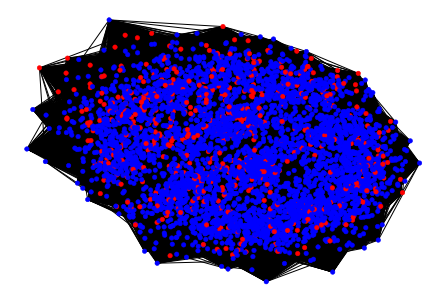
\includegraphics[width=0.5\textwidth]{Moro_network.png}
		\caption{MAG Graph of Bank Telemarketing Dataset}
        \label{fig:Moro}
	\end{figure}
  
  \noindent The red dots in figure \ref{fig:Moro} mark the clients which
  decided to invest in the short-term deposit and the blue dots did not invest.
  This figure masks some of the blue nodes due to the figure generation
  process. The general pattern however is apparent. The red nodes are randomly 
  placed in the network which suggests, that \acs{gml} will be of limited use. 
  The graph further shows, that only a relatively small number of clients appear 
  to have invested in the short-term deposit. To be more precise, only 
  approximately 12\% of bank clients invested in the short-term deposit. 
  The dataset is unbalanced which makes the classification task difficult.
  \acs{grl} using Node2Vec does not provide any useful results and 
  the \acsp{gnn} also perform rather poorly. In particular, \acsp{gnn} tend to 
  classify most clients as non-investors and struggle to accurately classify 
  clients which did invest. Due to the unbalanced data, it is loss optimizing 
  for the \acsp{gnn} to predict most nodes as non-investors rather than learning 
  the true label. Table \ref{table:Moro_conf} shows the confusion matrix of the 
  classification results for the validation dataset (20\%) using GraphSage.
  This model yielded the best results among the \acs{gml} models. 

  \begin{table}[h]
    \centering
    \begin{tabular}{|l|l|c|c}
      \hline
      \diagbox{\textbf{Label}}{\textbf{Predicted}} & \textbf{Did not invest} &
      \textbf{Invested} \\
      \hline
      \textbf{Did not invest} & 1'000 & 55 \\\hline 
      \textbf{Invested} & 104 & 54 \\
      \hline
    \end{tabular}
    \caption{Confusion Matrix Validation Bank Telemarketing Data}
    \label{table:Moro_conf}
  \end{table}

  \noindent The confusion matrix corresponds to an accuracy of approximately 
  86.89\%. The \acs{mag} generation process was repeated multiple times
  for which the GraphSage accuracies ranged between 86 - 90\%. Similar results
  are observed for both graph based methods and standard \acs{ml} modelss such 
  as \acsp{ann}, \acsp{svm}, and random forest classifiers. \\

  \noindent Unbalanced datasets are part of a larger and common problem in 
  \acs{ml}. Possible remedies might include using loss functions which 
  penalize false classifications harsher than the standard cross-entropy loss 
  function used for the \acsp{gnn}. Alternatively, one could also reduce the 
  dataset by dropping observations so that the remaining dataset is balanced. 
  This approach has its own problems as dropping a large number of observations 
  discards a lot of potentially valuable information. It could also put in 
  question the external validity of the model. These comments point to a 
  separate field of research and could be interesting for a future project. \\

  \noindent The failure using \acs{gml} models for this dataset reveals, that 
  \acsp{gnn} are not an easy remedy for unbalanced data. Perhaps, if the
  network structure provided clusters which corresponded to the labels,
  \acsp{gnn} could provide superior results. Given the variables available in 
  the dataset and the limitations of using the \acs{mag} model, this is not 
  possible. In order to check, whether network structure could indeed remedy 
  the unbalanced label problem, the label of the bank telemarketing dataset was 
  used as an additional attribute for the \acs{mag} model. The label is 
  normally not included as an attribute for the \acs{mag} model, as the label 
  data is usually unknown outside of the training dataset. The link-affinity 
  probabilities for the label is set as follows:

  \[ \Theta_{label} = 
	\begin{pmatrix}
        0.95 & 0.25 \\
		0.25 & 0.95 \\
	\end{pmatrix}
	\] 
  
  \noindent The resulting \acs{mag} which considers the label as an attribute 
  is shown in figure \ref{fig:Moro_bias}.

  \begin{figure}[h]
		\centering
		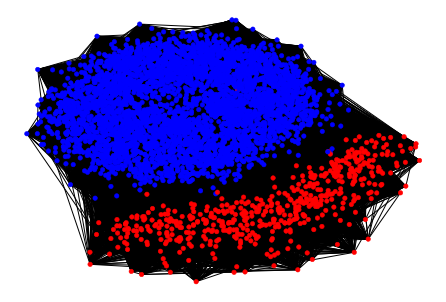
\includegraphics[width=0.5\textwidth]{Moro_network_bias.png}
		\caption{Biased MAG of the Bank Telemarketing Dataset}
        \label{fig:Moro_bias}
  \end{figure}

  \noindent The nodes shown in figure \ref{fig:Moro_bias} are now nicely
  clustered according to their label. The \acs{gnn} model GraphSage achieved an 
  accuracy of over 95\% for this graph using otherwise identical feature data
  and model specifications as before. This is of course a form of cheating, as 
  one cannot assume to know the labels of the graph outside of the training 
  setting. In a real-world application, the model would be trained using label
  data and then applied to new data which does not contain the label. This
  approach would however require the label for the graph generation procedure 
  which makes this not a viable approach. Nevertheless, this result shows 
  extremely well when \acs{gml} can yield superior results compared to standard 
  \acs{ml} models. The key lies in generating a graph with a network structure 
  that corresponds to the label. The network structure need not necessarily be 
  as clearly separated as shown in figure \ref{fig:Moro_bias}. A graph which 
  contains local neighborhood clusters which correspond to the same label could 
  yield similar good results. In such a setting, one would have to be careful 
  when defining the number of $K$ layers and the neighborhood sampling function 
  $\mathcal{N}_{k}$. A network structure which corresponds to the label could 
  perhaps also be generated without the label to an extent. This would require
  that the attribute data used in the \acs{mag} model to be related with the
  label. The attributes would have to be substitutes for generating a network
  structure which correspond to the label. Given the available attributes for
  the bank telemarketing dataset, this is a difficult task. All features in the 
  dataset have very low correlations with the label. The largest correlation, 
  which is a strong outlier, with the label is call duration with a correlation 
  coefficient $r\approx$ 0.4. This value is rather small and a simulation showed, 
  that it could not be used as a single substitute for the label. Selecting the
  appropriate attributes and defining the link-affinity probabilities is not a
  trivial task and requires a lot of trial and error. Unfortunately, for this
  dataset no appropriate attributes and link-affinities were found that yielded
  the desired result. For that reason, this dataset was also discarded for
  further analysis. The dataset and the performed analyses can be found in the 
  GitHub repository. 

  \section{US Airline Passenger Dataset}
  \label{section:airline_data}

  The \acs{us} airline passenger dataset is a survey which was conducted in 2015
  by J.D. Power \citeyearpar{JDPower2015}. The dataset was retrieved on the 
  website Kaggle \citeyearpar{KAGGLE2015} and is well suited for applying 
  \acs{gml} following the \acs{mag} generation procedure. The dataset focuses on 
  classifying satisfied- and neutral or dissatisfied passengers. The dataset is 
  thus set up for a standard binary classification task. The dataset further 
  proves to be a competitive dataset for standard \acs{ml} models. This makes 
  this dataset a suitable candidate for a fair comparison of \acs{gml} vs. 
  standard \acs{ml}. This dataset is presented in detail as it is used for the 
  results shown in chapter \ref{section:results}. \\

  \noindent An overview of the \acs{us} airline passenger dataset is shown in 
  table \ref{table:airline_summary}. The correlation heatmap of the dataset is
  further shown in figure \ref{fig:corr_heatmap}. The correlation heatmap
  reveals, that the variables "departure delay in minutes" and "arrival delay
  in minutes" are highly correlated. As "arrival delay in minutes" has some
  missing observations, this variable is dropped in favor of "departure delay 
  in minutes". The heatmap and its corresponding correlation matrix reveal,
  that "gender" is approximately uncorrelated with any of the other variables.
  Further, "departure delay in minutes" appears to be approximately uncorrelated 
  with any of the other variables. For that reason, it was tested whether both 
  variables could be excluded. The results however reveal, that the \acs{ml} 
  models performed better if these variables are included in the model. The data 
  shown in table \ref{table:airline_summary} and figure \ref{fig:corr_heatmap} 
  corresponds to a random sample of 6’000 observations from the training dataset 
  consisting of 103’904 observations. The training graph is created using this 
  sample of 6'000 observations due to computational time considerations.
  Several random samples were used to generate \acsp{mag}, for which the
  results of all simulations were consistent.

  \begin{figure}[h]
	  \centering
	  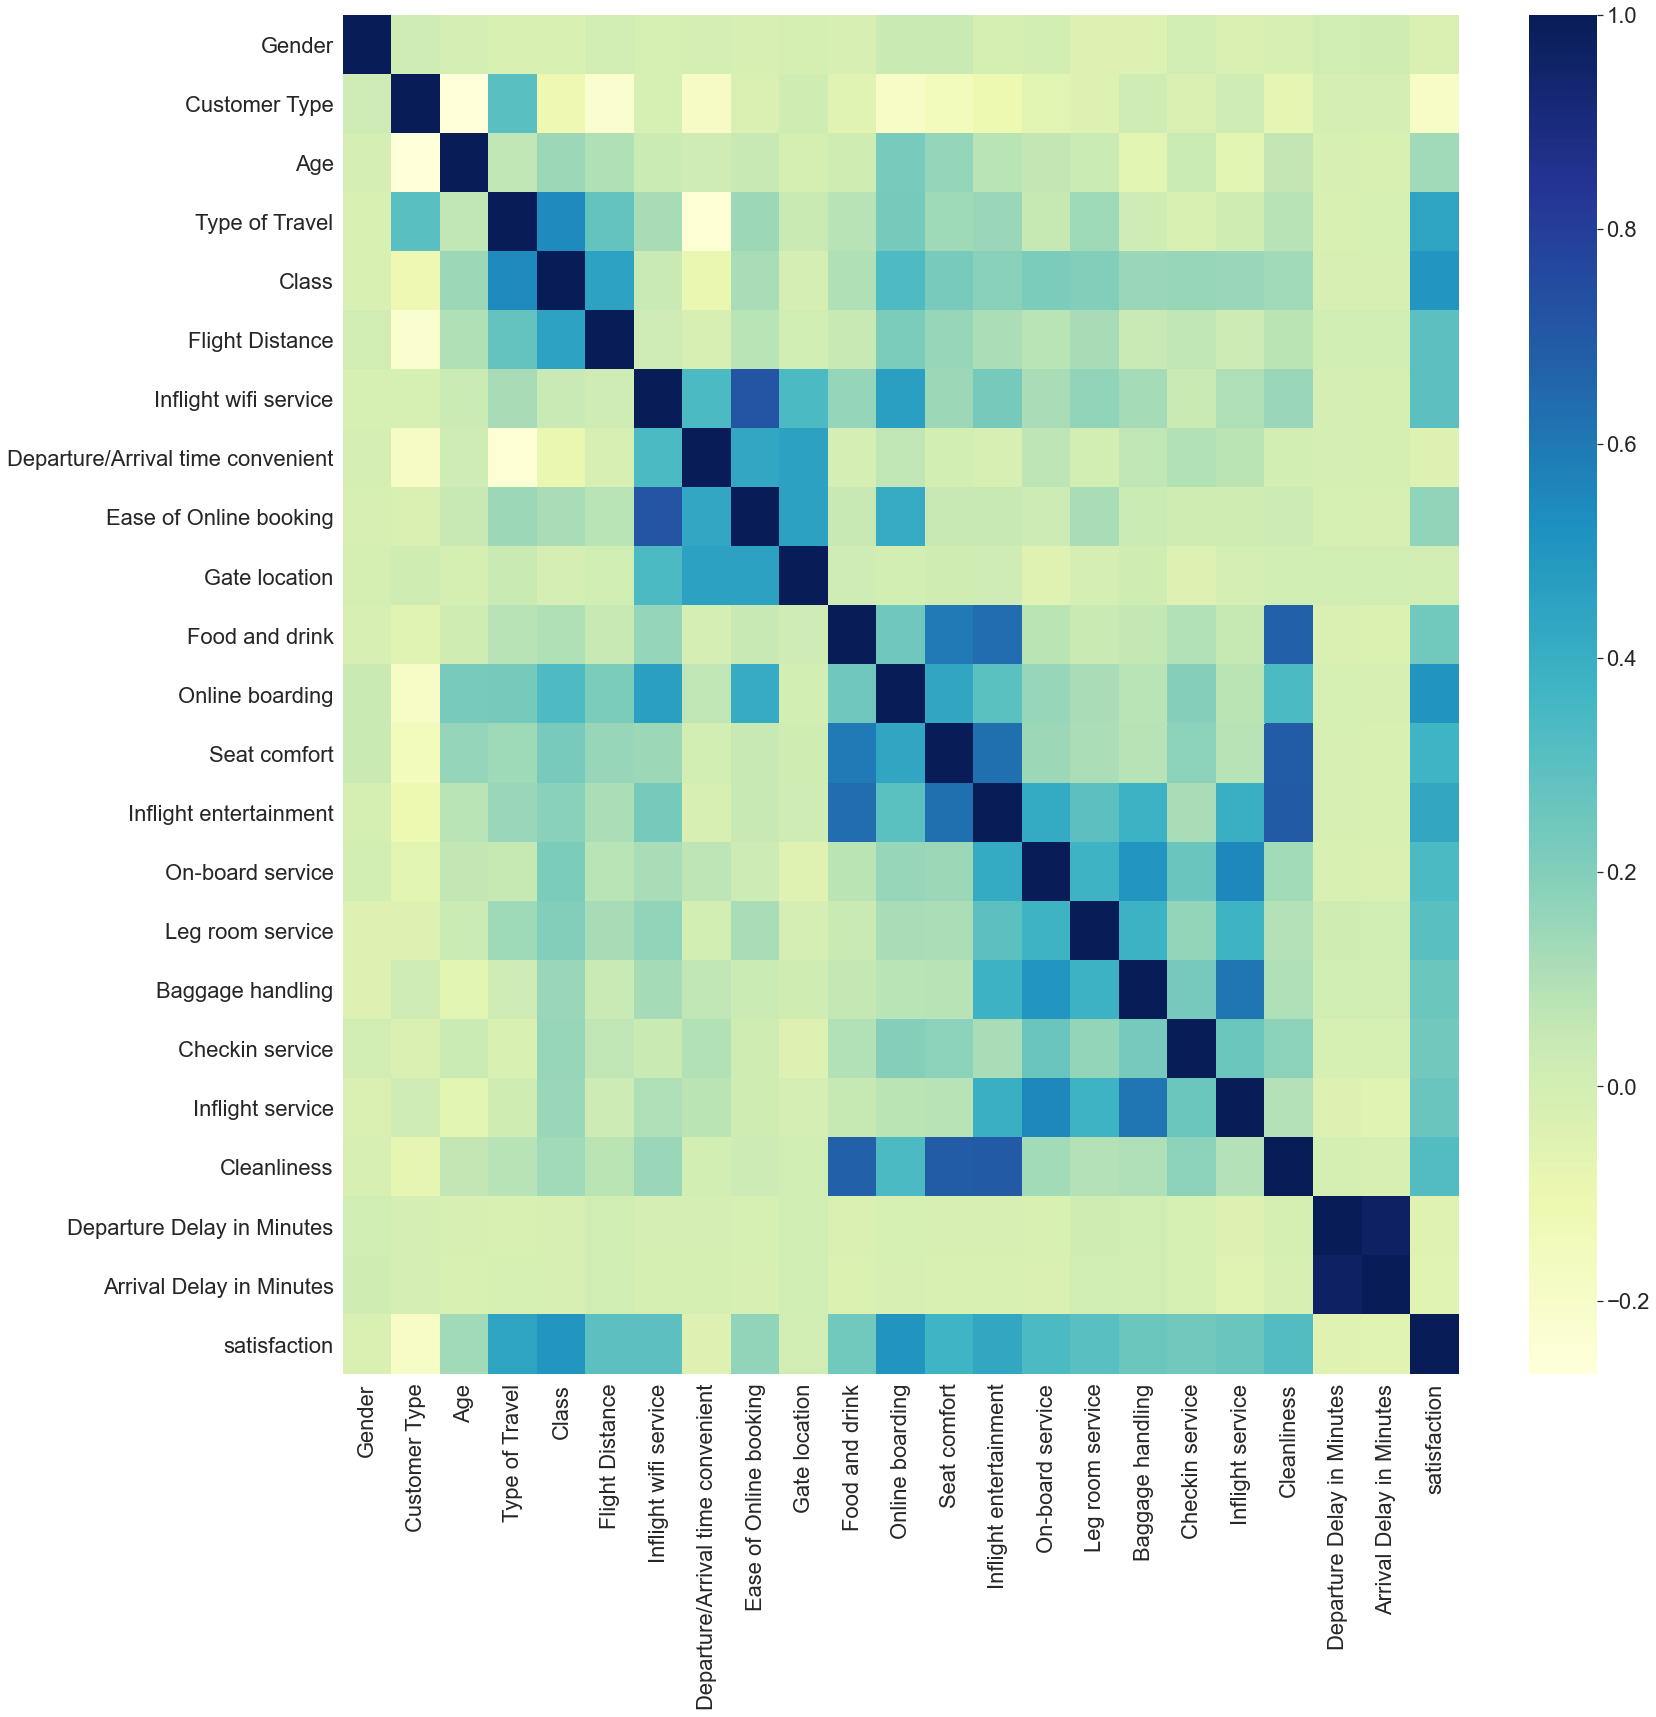
\includegraphics[width=1.0\textwidth]{corr_heatmap.png}
	  \caption{Correlation Heatmap of US Airline Passenger Dataset}
      \label{fig:corr_heatmap}
  \end{figure}

  \begin{landscape}
  \pagestyle{empty}
  \begin{table}[h]
    \centering
    \begin{tabular}{|l|L|c|c|}
      \hline
      \textbf{Variable} & \textbf{Description} & \textbf{Mean} & \textbf{Range} \\
      \hline
      Satisfaction (label) & Satisfaction: Airline satisfaction level (satisfied:1, 
      neutral or dissatisfied:0) & 0.4295 & 0 - 1 \\\hline
      Gender & Gender of the passengers (male:0, female:1) & 0.5076 & 0 - 1
      \\\hline 
      Customer Type & The customer type (loyal customer:0, disloyal customer:1) 
      & 0.18 & 0 - 1 \\\hline
      Age & The actual age of the passengers & 39.101 & 7 - 85 \\\hline
      Type of Travel & Purpose of the flight of the passengers
      (personal travel:0, business travel:1) & 0.6891 & 0 - 1 \\\hline
      Flight Distance & The flight distance of this journey &
      1'197.438 & 67 - 4'963 \\\hline
      Departure Delay in Minutes & Minutes delayed when departure & 14.808 & 0 - 595 \\\hline
      Arrival Delay in Minutes & Minutes delayed when arrival & 15.159 & 0 -
      589 \\\hline
      Class & Travel class in the plane of the passengers (Eco:1, Eco Plus:2, 
      Business:3) & - & 1 - 3 \\\hline
      Inflight WiFi service & Satisfaction level of the inflight WiFi service
      (0:not applicable;1-5) & - & 0 - 5 \\\hline
      Ease of Online booking & Satisfaction level of online booking & - & 0 - 5
      \\\hline
      Gate location & Satisfaction level of gate location & - & 0 - 5 \\\hline
      Food and drink & Satisfaction level of Food and drink & - & 0 - 5
      \\\hline
      Online boarding & Satisfaction level of online boarding & - & 0 - 5
      \\\hline
      Seat comfort & Satisfaction level of seat comfort & - & 0 - 5 \\\hline
      Inflight entertainment & Satisfaction level of inflight entertainment & -
                             & 0 - 5 \\\hline
      On-board service & Satisfaction level of on-board service & - & 0 - 5
      \\\hline
      Leg room service & Satisfaction level of leg room service & - & 0 - 5
      \\\hline
      Baggage handling & Satisfaction level of baggage handling & - & 0 - 5
      \\\hline
      Check-in service & Satisfaction level of check-in service & - & 0 - 5
      \\\hline
      Inflight service & Satisfaction level of inflight service & - & 0 - 5
      \\\hline
      Cleanliness & Satisfaction level of cleanliness & - & 0 - 5 \\
      \hline
    \end{tabular}
    \caption{US Airline Passenger Dataset}
    \label{table:airline_summary}
  \end{table}
  \end{landscape}

  \noindent The variables of the dataset are categorized as follows:

  \begin{itemize}
    \item \textbf{Categorical Variables:} Gender, Customer Type, Type of 
      Travel, and Satisfaction
    \item \textbf{Ordinal Variables:} Class, Inflight WiFi Service, Ease of Online
      Booking, Gate Location, Food and Drink, Online Boarding, Seat Comfort,
      Inflight Entertainment, On-Board Service, Leg Room Service, Baggage
      Handling, Check-in Service, Inflight Service, and Cleanliness
    \item \textbf{Numerical Variables:} Age, Flight Distance, and 
      Departure Delay in Minutes
  \end{itemize}

  \noindent The categorical variables are dummy coded and the ordinal variable
  class is coded as shown in table \ref{table:airline_summary}. The remaining 
  ordinal variables which measure different satisfaction levels are recorded 
  using a Likert scale ranging from $1 - 5$. Many passengers did not answer all 
  satisfaction level questions. These responses are recorded with a 0. Therefore, 
  the range of values for the satisfaction level variables range from $0 - 5$. 
  This encoding works well, as a 0 input in a linear pass function of a (graph) 
  neural network will result in a 0 output value. This type of encoding allows 
  for dealing with missing values for neural networks and other \acs{ml}
  models. Lastly, the numerical variables had to be normalized. The popular 
  approach of standardizing the entire dataset was unfortunately not possible. 
  Due to the missing values prevalent in the satisfaction level variables, it 
  must be ensured, that a 0 refers to as a missing response. Note, that a 
  recorded 0 for the numerical variables does not correspond to a missing value. 
  For that reason, the min-max normalizing function was applied and is defined 
  as follows:

  \begin{equation}
    x' = a + \frac{(x - \min(x))(b - a)}{\max(x) - \min(x)}
    \label{eq:norm}
  \end{equation}

  \noindent In equation \ref{eq:norm}, $x$ refers to the unnormalized 
  variable and $x'$ refers to resulting normalized variable. $a$ defines 
  the lower bound of the normalization range and $b$ is the upper bound. The
  numerical variables are normalized to be within the range $[1,5]$. Now, all 
  variables are within a similar range and different scaling should no longer 
  lead to biasing behavior. \\

  \noindent In the following section, the graph generation process for the
  \acs{us} airline passenger dataset is described in detail.

  \subsection{Graph Generation}
  \label{section:graph_gen}

  To create a graph from the US airline passenger dataset, appropriate
  attributes must be selected for the \acs{mag} model. The selected attributes 
  must be of a type such that realistic probabilities can be assigned. As an 
  example, it is difficult to assign link-affinity probabilities for people who 
  gave ratings regarding the "inflight wifi service". In this case one could 
  assign a probability that people who gave high ratings are more similar with 
  relative ease. However, does this then also translate to people not liking 
  the wifi-service being similar as well? Further, how do we assign 
  probabilities for people who are dissimilar? These considerations make the 
  selection of appropriate attributes difficult. It is therefore important to 
  select attributes for which realistic probabilities for all of the following
  three settings can be assigned:

  \begin{itemize}
    \item \textbf{Positive similar observations} (e.g. both observations like 
      the service)
    \item \textbf{Negative similar observations} (e.g. both observations 
      dislike the service)
    \item \textbf{Dissimilar observations} (Symmetric for undirected graphs, 
      can be asymmetric for directed graphs)
  \end{itemize}
 
  \noindent The attributes are selected using the above mentioned considerations. 
  The selected attributes with the corresponding link-affinity probabilities are 
  shown in table \ref{table:link_aff}.

  \begin{table}[h]
    \centering
    \begin{tabular}{|l||L|}
      \hline
      \textbf{Attribute Name} & \textbf{Link-Affinity Probabilities}\\
      \hline\hline
      Gender & 0.6, 0.4; 0.4, 0.6  \\\hline 
      Customer Type & 0.8, 0.5; 0.5, 0.8 \\\hline
      Age & 0.90, 0.80, 0.60, 0,40; 0.80, 0.90, 0.80, 0.60; 0.60, 0.80, 0.90,
      0.80; 0.40, 0.60, 0.80, 0.90 \\\hline
      Type of Travel & 0.80, 0.20; 0.20, 0.80 \\\hline
      Class & 0.85, 0.60, 0.45; 0.60, 0.85, 0.60; 0.45, 0.60, 0.85 \\
      \hline
    \end{tabular}
    \caption{Link-Affinity Matrices}
    \label{table:link_aff}
  \end{table}

  \noindent The probabilities in table \ref{table:link_aff} correspond to the
  rows of the link-affinity matrices up to the semi-colon. To give a better
  overview, the link-affinity matrix for age is shown explicitly as follows:

  \[ \Theta_{Age} = 
	\begin{pmatrix}
		0.90 & 0.80 & 0.60 & 0.40 \\
        0.80 & 0.90 & 0.80 & 0.60 \\
        0.60 & 0.80 & 0.90 & 0.80 \\
        0.40 & 0.60 & 0.80 & 0.90 \\
	\end{pmatrix}
  \] 

  \noindent The attribute age has a rather large cardinality which makes it 
  difficult to use for the \acs{mag} model. For that reason, age is binned into 
  4 categories with 0 if age $<$ 26, 1 if 26 $\leqslant$ age $<$ 39, 2 if 39 
  $\leqslant$ age $<$ 50, and 3 if age $\geqslant$ 50. These bins are chosen 
  according to the interquartile lengths present in the distribution of the 
  attribute age. The transformed attribute now contains 4 categories and now
  matches the link-affinity matrix shown above.\\

  \noindent There exist no clear rules for assigning link-affinity
  probabilities. \citeauthor{kim2012multiplicative} 
  \citeyearpar[p. 118]{kim2012multiplicative} presented the 4 common 
  link-affinity matrix structures of homophily, heterophily, core-periphery, and 
  random for creating graphs. Given the selected attribute data, the homophily 
  setting appears to be most appropriate for all link-affinity matrices. In this 
  setting, observations which are similar have a higher probability of forming a 
  connection compared to dissimilar observations. It can however not be ruled out, 
  that different link-affinity matrix structures might be more appropriate. The 
  probabilities shown in table \ref{table:link_aff} were chosen based on 
  personal intuition and trial and error. To test this, several graphs were 
  created using different probabilities. The homophily structure with the 
  probabilities shown in table \ref{table:link_aff} generated the best 
  graphs. There is however no exact science or selection criteria which can be 
  applied for selecting attributes and defining the link-affinity probabilities. \\

  \noindent As mentioned in the previous section, a sub-sample of 6'000 
  observations was retrieved from the training dataset consisting of 103’904 
  observations. With this random subsample and the attributes shown in table
  \ref{table:link_aff}, the adjacency matrix for the resulting graph $G(V,E)$ 
  is generated using algorithm \ref{algo:MAG}. The random subsample is 
  retrieved due to the computational cost of running algorithm \ref{algo:MAG}. 
  Simulations which involved creating graphs with different random subsamples 
  show, that the random subsamples are representative for the entire dataset. 
  This is further supported when comparing the summary statistics of the 
  subsamples with the full dataset. The generated graph is shown in figure 
  \ref{fig:us_airline_graph}.

  \begin{figure}[h]
	  \centering
	  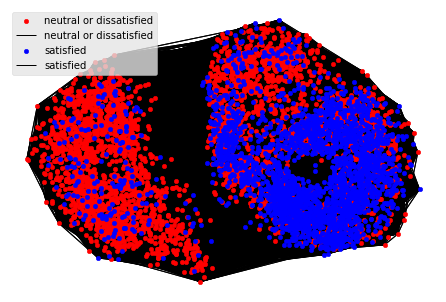
\includegraphics[width=0.5\textwidth]{us_airline_graph.png}
	  \caption{Graph of US Airline Passenger Dataset}
      \label{fig:us_airline_graph}
  \end{figure}
  
  \noindent The network in figure \ref{fig:us_airline_graph} shows the 
  emergence of two primary clusters. In addition one can see, that most satisfied 
  airline passengers appear to be grouped together in the right cluster. To 
  gain a deeper understanding of the dynamics involved in the network formation, 
  the nodes of the network are plotted excluding the edges in figure
  \ref{fig:us_airline_nodes}.

  \begin{figure}[h]
	  \centering
	  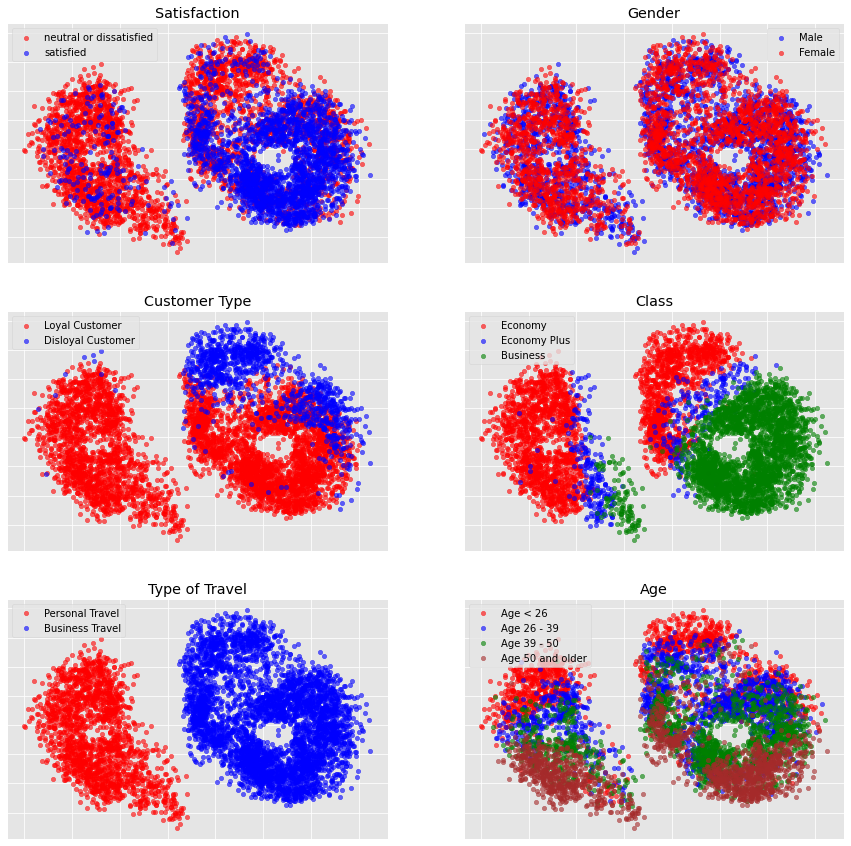
\includegraphics[width=0.8\textwidth]{us_airline_nodes.png}
	  \caption{Graph Nodes of US Airline Passenger Dataset}
      \label{fig:us_airline_nodes}
  \end{figure}

  \noindent Figure \ref{fig:us_airline_nodes} plots the nodes of the network
  for the label satisfaction and the 5 attributes used for the graph
  generation. The transparency of the plot is set to $\alpha = 0.6$ to avoid 
  covering nodes during the graph plotting process. Figure
  \ref{fig:us_airline_nodes} reveals interesting associations. First it is
  shown, that a larger number of people traveling for business purposes are 
  satisfied compared to people traveling for personal reasons. This association
  becomes clear when comparing the satisfaction plot with the type of travel
  plot. In relative terms, only approximately 9.8\% of passengers traveling for 
  personal reasons are satisfied compared to business travelers with a 57.8\% 
  satisfaction rate. Interestingly, passengers traveling for business purposes
  adhere to somewhat expected characteristics such as:

  \begin{enumerate}
    \item Most business class passengers are satisfied. 
    \item Older passengers appear to be more satisfied which is largely
      associated with booking more business class tickets. The age plot however 
      reveals, that older passengers tend to be mostly satisfied even when 
      booking economy class.
    \item Most loyal customers book business class. There is some overlap where 
      loyal customers also book economy class tickets. The reverse is true as 
      well, where a cluster of disloyal customers book business class. 
  \end{enumerate}
  
  \noindent Passengers traveling for personal reasons do not appear to adhere
  to the characteristics or associations shown for business travelers. The only
  distinctive character is, that almost all passenger traveling for personal
  reasons are loyal customers. This fact does however not appear to be
  associated with satisfaction. At first, this seems like a rather bizarre 
  finding. Upon further reflection, this could point to a sampling bias of 
  passengers traveling for personal reasons due to following considerations:

  \begin{enumerate}
    \item It is reasonable that almost only loyal passengers participated. When 
      traveling, most people do not participate in surveys. This is especially 
      true for disloyal customers. Business travelers for comparison might give
      routine feedback due to company policies.
    \item It is common, that dissatisfied people are more likely to give
      feedback, while satisfied passengers are less likely to participate in
      the survey. Again, the data regarding business travelers might be more
      reliable here due to company mandated survey participation.
    \item Perhaps business travelers fly more frequently than passengers
      traveling for personal reasons. This could incentivize frequent business
      travelers to give feedback as they would benefit most from service
      improvements. Infrequent personal travelers might be less incentivized,
      as they benefit less from service improvements. 
  \end{enumerate}

  \noindent Last but not least, gender does not appear to form any distinguishable 
  clusters. For that reason, it was considered to omit this attribute for the 
  graph generation process. This was tested and the resulting graph was similar
  to the one shown in figure \ref{fig:us_airline_graph}. The graph was however 
  more spread out and the neighborhood structures were less clear. In addition, 
  the graph without gender did not perform as well in the subsequent machine 
  learning tasks. Gender appears to provide some useful network information 
  which is why the attribute is kept for the graph generation process. \\

  \noindent To provide some more context regarding the graph structure, some
  graph theoretical metrics are provided. The degree distribution as well as 
  the distributions of the centrality measures: eigenvector centrality, 
  closeness centrality, and betweenness centrality are shown in 
  figure \ref{fig:centrality_measures}.

  \begin{figure}[h]
	  \centering
	  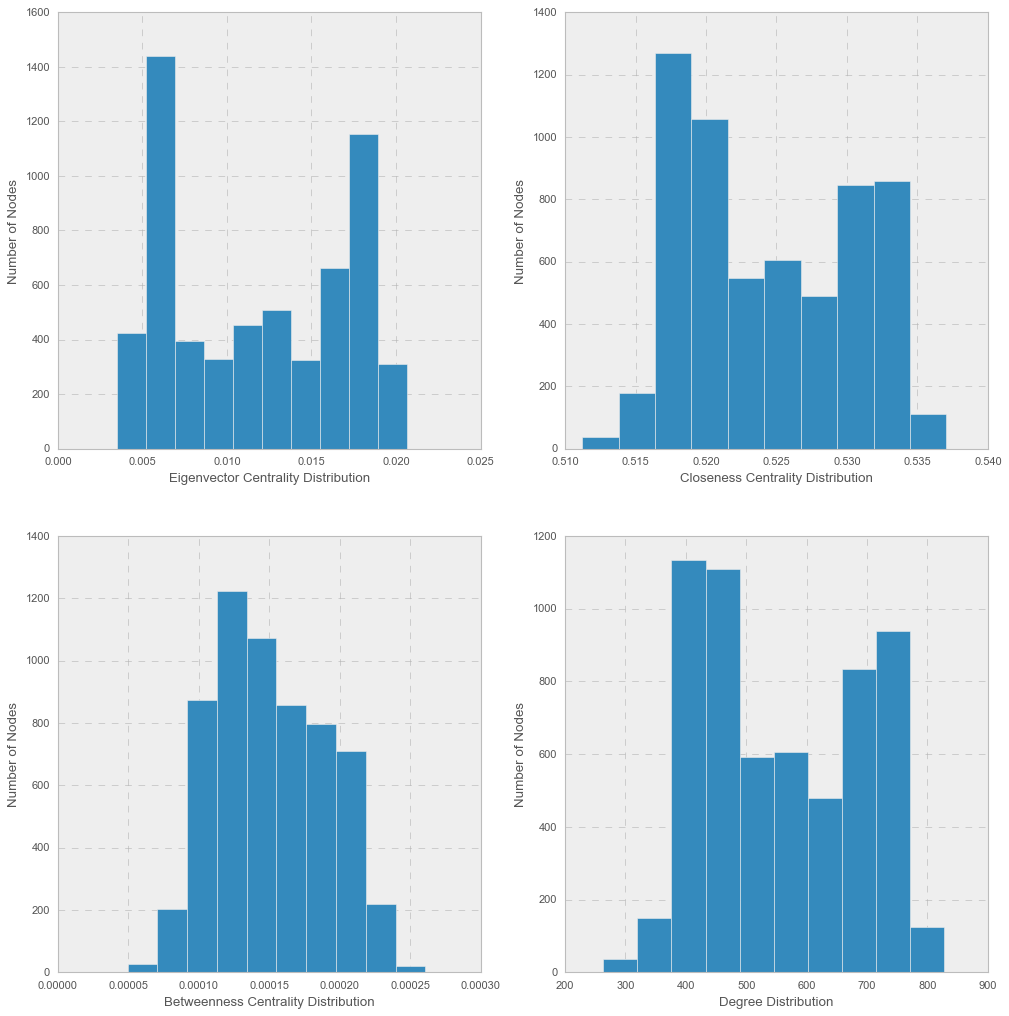
\includegraphics[width=0.7\textwidth]{centrality_measures.png}
	  \caption{Graph Statistics}
      \label{fig:centrality_measures}
  \end{figure}

  \noindent The network has a density of approximately 0.0933. This means that 
  9\% of the potential number of connections formed in the network.
  Nevertheless, when looking at the degree distribution histogram we can see, 
  that all nodes have a large number of connections ranging between 263 -
  828 with an average of 559.63 connections. The distribution has two
  modes which likely correspond to the two main clusters shown in figure
  \ref{fig:us_airline_nodes}. The eigenvector centrality distribution shows, 
  that all nodes have a very low centrality measure and therefore none of the 
  nodes appear to have a large impact in terms of eigenvector centrality. The 
  closeness centrality distribution shows, that all nodes have an average 
  closeness centrality ranging from 0.51 - 0.53. This means that every node is 
  similarly connected and has an average impact for disseminating information 
  across the network. Lastly, the betweenness centrality distribution reveals 
  that there are no bottle-necks through which information flows. \\

  \noindent As a reference point, it is important to compare the properties of
  the created graph to real world graphs. \acsp{gnn} were designed with real
  world networks in mind. Especially the large number of vertex degrees might
  be of concern and is discussed in more detail in section 
  \ref{section:gml_performance}. For that reason, the generated \acs{mag} is
  compared to real networks. The most appropriate type of networks for comparison 
  are a social networks. Common structures of social networks include 
  \citep{watts1998collective,newman2006structure,Newman2010,kim2012multiplicative}:

  \begin{enumerate}
    \item Degree distributions often follow a power law distribution
    \item Emergence of a giant connected component
    \item Core-periphery structure
  \end{enumerate}

  \noindent The power law degree distribution and the emergence of a giant
  connected component creates network structures that have an onion
  (core-periphery) structure \citep[p. 121]{kim2012multiplicative}. This
  indicates, that most social networks have a few very highly connected nodes
  and many nodes with few connections. This creates a right skewed degree 
  distribution which also leads to a right skewed eigenvector centrality and
  closeness centrality distribution. For the betweenness centrality it is 
  also expected, that more central nodes in a core-periphery network structure
  would exhibit some bottleneck properties for the central nodes. For that
  reason one would expect central nodes to have a higher betweenness centrality.
  When looking at the distributions in figure \ref{fig:centrality_measures},
  this does not correspond to a power law degree distribution. The centrality 
  measures further do not correspond to the centralities frequently observed in 
  real social networks. The graph created with the \acs{mag} model does therefore 
  not share the properties observed in real social networks. In order to 
  generate a graph which shares the properties of real networks, one would have 
  to adapt the link-affinity properties to the core-periphery setting as shown 
  in figure \ref{fig:link-affinity}. This was tested and indeed an onion shaped
  network was created using the same attributes. Forcing this core-periphery 
  structure is however not purposeful for this thesis. This would require
  setting link-affinity probabilities for the feature data which would not make
  sense. Further, the aim of this thesis is not necessarily to create realistic 
  graphs rather than to create useful graphs for \acs{gml}. The results in 
  chapter \ref{section:results} reveal, that the graph is indeed useful for
  \acs{ml}. For that reason, the generated graph shown in this section was kept 
  for further analysis. 

  \subsection{Stochastic vs. Deterministic MAGs}
  \label{section:stoch_det}

  In section \ref{section:self_survey}, the question was raised 
  as to whether the \acs{mag} should form connections between observations
  stochastically or whether a deterministic threshold probability yields better 
  results. In the previous sections, the graphs were generated stochastically.
  In this section, the \acs{us} airline passenger dataset is used for 
  generating a deterministic graph. The first insight gained when investigating 
  this question lies in the fact, that the probability of two observations is 
  generally very low. When setting the threshold probability for a connection 
  between two observations $u$ and $v$ to 0.5, not a single connection is made. 
  This follows, as the probability for a connection decreases by design as the 
  number of attributes increases. This is implicitly shown in equation 
  \ref{eq:MAG}, where the product of probabilities is bound to approach 0 as
  the number of attributes increases. For this reason, it is suggested to limit 
  the number of attributes to $K=\rho\log_{2}N$ for some constant $\rho$ 
  \citep[p. 122]{kim2012multiplicative}. The number of attributes are selected 
  accordingly such that $K\leqslant\log_{2} N$. The threshold probability for a 
  connection was set to 0.2 in the \acs{mag} model. The \acs{mag} yielded 
  several disconnected graphs which are for the most part clustered according to 
  their group memberships. Figure \ref{fig:det_MAG} shows the graphs for the 
  label and the attributes, where the edges are removed. The subgraphs are 
  unfortunately plotted very small, however all graphs combined include all 
  6'000 nodes. The plots are meant to provide a high-level overview of the 
  generated subgraphs. 

  \begin{figure}[h]
		\centering
		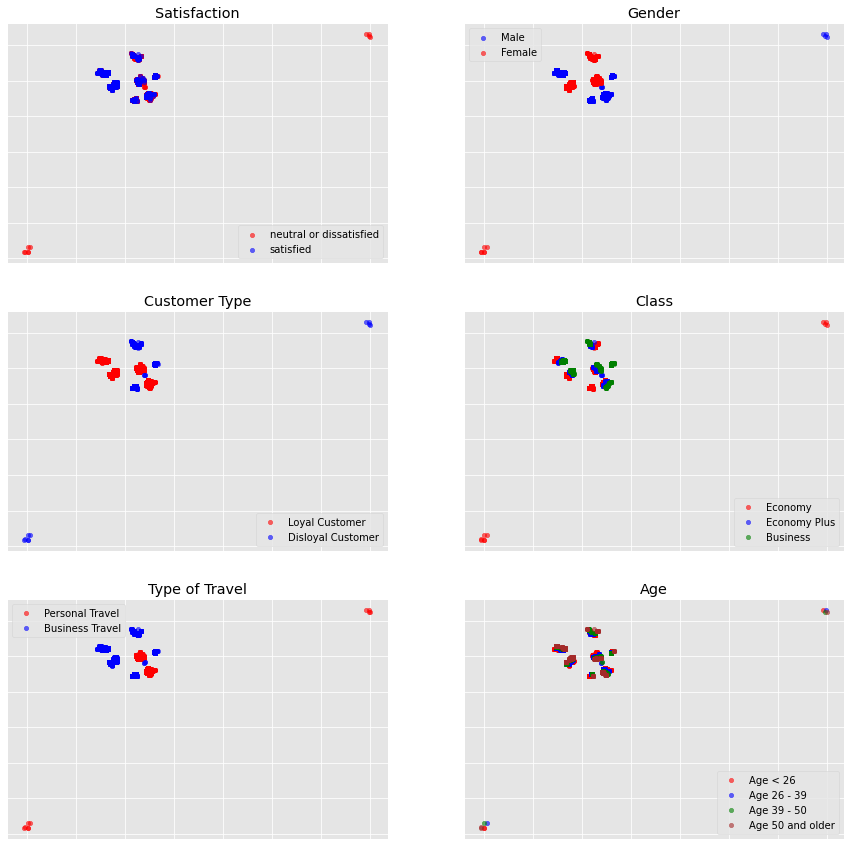
\includegraphics[width=1.0\textwidth]{deterministic_MAG.png}
		\caption{Deterministic MAG graph}
        \label{fig:det_MAG}
  \end{figure}

  \noindent The deterministic \acs{mag} model crates disconnected graphs which 
  form clusters based on node similarities. In terms of performance, the accuracy 
  and loss behavior of both the deterministic- and stochastic generated graphs 
  were virtually identical. The \acs{gml} results using GraphSage for the
  deterministic \acs{mag} is shown in appendix \ref{app:det_graphs}. For the 
  purpose of visualization, stochastic graphs are more useful, as one can 
  identify the different clusters and their relationships to one another on a 
  single connected graph. For this reason, the stochastic graph generation 
  process is kept. Nevertheless, deterministic graph generation appears to be 
  useful if one wants to separate nodes into more homogeneous subgraphs. These 
  subgraphs could then be used for subsequent \acs{ml} tasks with a cluster 
  specific task in mind. The clusters further could provide information as to 
  which clusters tend to be more or less satisfied. This is an area which could 
  be interesting for future research.
  
